\documentclass{article}
\usepackage[utf8]{inputenc}
\usepackage[T1]{fontenc}
\usepackage{graphicx} % handles figures
\usepackage[fleqn]{mathtools}
\usepackage{amsmath}
\usepackage{hyperref}
\usepackage{amssymb}
\usepackage{xcolor}

%Insertion de tout un tas de librairie qui nous seront probablement inutiles pour la pluspart mais it's always good to have them
\title{\textbf{Maths Discrètes}\\ Solutions TP 7}
\date{}
\begin{document}
\maketitle % fais le titre écris plus haut


\section*{Exercice 1}
\begin{align*}
\underset{i=0}{\overset{n}{\sum}}\underset{j=0}{\overset{i}{\sum}}\binom{n}{i}\binom{i}{j} &=
\underset{i=0}{\overset{n}{\sum}}\binom{n}{i}
\begin{pmatrix}
\underset{j=0}{\overset{i}{\sum}}\binom{i}{j}
\end{pmatrix} \\ &=
\underset{i=0}{\overset{n}{\sum}}\binom{n}{i} (1+1)^{i} \\&=
(2+1)^{n} \\ &=
3^{n}
\end{align*}

\section*{Exercice 2}
\begin{align*}
\underset{i=0}{\overset{n}{\sum}}
\begin{pmatrix}
n+1 \\
i+1
\end{pmatrix}
(i+1)2^{i} &=
\underset{i=0}{\overset{n}{\sum}}(n+1)\dfrac{n!}{i!(n-i)!}2^{i} \\ &=
(n+1)(2+1)^{n} \\ &=
3^{n}(n+1)
\end{align*}

\section*{Exercice 3}
\begin{itemize}
\item $8, 2, 8, 2, 8, 2$ 
\item $9, 4, 10, 13, 1, 10, 1, 10, 4, 8, 1, 13, 9$
\end{itemize}

\section*{Exercice 4}
\begin{enumerate}
\item 
\begin{alignat*}{10}
&2 \hspace{1pt}\rule{10pt}{1pt} \hspace{1pt}&&4\hspace{1pt}\rule{10pt}{1pt} \hspace{1pt}&&1\hspace{1pt}\rule{10pt}{1pt}\hspace{1pt} &6\\
& && &&\hspace{1pt}\rule{1pt}{10pt} &\\
& && &&3 \hspace{1pt}\rule{10pt}{1pt} &5
\end{alignat*}
\item
\begin{alignat*}{10}
&5 \hspace{1pt}\rule{10pt}{1pt} \hspace{1pt}&&3 \hspace{1pt}\rule{10pt}{1pt} \hspace{1pt}&&6 \hspace{1pt}\rule{10pt}{1pt}\hspace{1pt} &2\hspace{1pt}\rule{10pt}{1pt}\hspace{1pt} &1 \hspace{1pt}\rule{10pt}{1pt}\hspace{1pt} &4 \hspace{1pt}\rule{10pt}{1pt}\hspace{1pt} &8\\
& && &&\hspace{1pt}\rule{1pt}{10pt} &\\
& && &&7
\end{alignat*}
\end{enumerate}

\section*{Exercice 5}
voir page suivante.

\section*{Exercice 6}
Algorithme pour Prüfer (Wikipédia les enfants!)

\section*{Exercice 7}
Un vecteur de degré contient les degrés de chaque sommet d'un graphe:
\begin{align*}
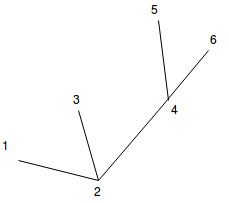
\includegraphics[scale=0.3]{exo7.jpg}
\Rightarrow (1, 3, 1, 3, 1, 1)
\end{align*}

\textit{La suite est à prendre avec des pincettes, je n'ai pas pris le temps d'y réfléchir donc c'est du décodage de notes pas très claires - si vous avez plus d'idées que moi je suis tout ouïe.}
\begin{align*}
\text{Donc la somme des degrés } & \text{des $n$ sommets est }
\underset{i=0}{\overset{n}{\sum}}\phantom{a}d_{i}-1 = n-2  \text{ donc:}\\
(n \times 1)^{n-2} &= \underset{k=0}{\overset{n-2}{\sum}}\begin{pmatrix}
n-2\\
k
\end{pmatrix}n^{k}\phantom{a}1^{n-k}\\
& = \underset{k=0}{\overset{n-2}{\sum}}\begin{pmatrix}
n-2\\
k
\end{pmatrix}n^{k}\\
& = \underset{(d_1,...,d_n)}{\sum}\begin{pmatrix}
n-2\\
d_1 -1 ,...,d_n - 1
\end{pmatrix}\\
\end{align*}


\end{document}
